\chapter{Introducción a los sistemas de comunicación}

\section{Introducción}

Desde el principio de los tiempos, el ser humano se ha comunicado con sus congéneres de distintas maneras: comenzó a través de la voz (se cree que hace unos 100.000 años), con algún tipo de protolenguaje, para posteriormente comenzar a utilizar sistemas de comunicaciones permanentes.

Por todos es conocido la evolución histórica de distintos sistemas escritos, entre los que podemos destacar (\href{https://es.wikipedia.org/wiki/Anexo:Cronolog%C3%ADa_de_las_tecnolog%C3%ADas_de_la_comunicaci%C3%B3n}{referencia}):
\begin{itemize}
    \item \textbf{Pinturas rupestres}: Realizadas en cuevas o rocas en las que se pueden observar escenas de caza, distintos animales, grabado de manos, figuras humanas... Algunas de las pinturas encontradas cuentan con más de 50.000 años. Tenemos un ejemplo cercano en las \href{https://es.wikipedia.org/wiki/Cueva_de_Santimami\%C3\%B1e}{cuevas de Santimamiñe} en donde tenemos pinturas datadas entre 14.000 y 9.000 años a. C.

    \item \textbf{Escritura cuneiforme}: Es uno de los primeros sistemas de escritura realizados, y se utilizaban tablillas de arcilla húmeda en las que se grababa mediante un tallo vegetal. Con este sistema se han datado tablas anteriores al 3.200 a.C. y en distintos idiomas.

    \item \textbf{Escritura jeroglífica y el papiro}: En el antiguo Egipto se crea la escritura mediante signos que comienza por escribirse en paredes para posteriormente inventar el papiro (cuya datación más antigua es del 2.500 a.C.) y de esta manera se comienza a tener un sistema de comunicación fácilmente manejable e intercambiable.

    \item \textbf{Uso de palomas mensajeras}: El uso de palomas mensajeras para el envío de comunicaciones data de la época anterior a 1.500 a.C. y se ha estado utilizando hasta este siglo en algunos países durante desastres naturales.

    \item \textbf{Telégrafo}: A partir de mediados del siglo XVIII y durante el inicio del siglo XIX hubo bastantes avances en las investigaciones del electromagnetismo y de esta manera se comenzó a investigar cómo usarlo para el envío de señales. En 1837 Samuel Morse patenta el \href{https://es.wikipedia.org/wiki/Tel%C3%A9grafo#Historia_del_tel%C3%A9grafo}{telégrafo}. En 1858 se une Irlanda y Terranova mediante el primer cable trasatlántico.

    \item \textbf{Teléfono}: Como evolución al telégrafo, que sólo permitía el envío de señales, nace el teléfono de la mano de \href{https://es.wikipedia.org/wiki/Antonio_Meucci}{Antonio Meucci} (aunque normalmente se le atribuye el invento a \href{https://es.wikipedia.org/wiki/Alexander_Graham_Bell}{Alexander Graham Bell}). En 1860 realizó una demostración pública transmitiendo voz a una considerable distancia.
\end{itemize}

Tal como podemos ver, ha habido distintos sistemas de comunicación utilizados durante siglos para el envío y recepción de información.

\section{Comunicación de la información}

Tal como hemos visto, los sistemas de comunicación de la información no es algo nuevo, ¿pero qué necesidades tiene un sistema de comunicación?

\begin{itemize}
    \item \textbf{Emisor}: Es el origen y la fuente de la información que se pretende comunicar.
    \item \textbf{Receptor}: Es el destinatario, el que va a recibir la información.
    \item \textbf{Mensaje}: Es la información que queremos transmitir entre el emisor y el recepetor.
    \item \textbf{Código}: Es el conjunto de reglas utilizadas a la hora de representar el mensaje. El emisor y receptor deben utilizar el mismo código para que la comnunicación sea correcta.
    \item \textbf{Canal}: Es el medio físico por el que se va a enviar el mensaje.
    \item \textbf{Señal}: Es el componente físico por el que se envía la información.
\end{itemize}

Para entender de mejor manera un sistema de comunicación y los componentes que lo forman, vamos a poner dos ejemplos:

\subsubsection*{Ejemplo 1: Comunicación oral}

\begin{wrapfigure}{r}{0.25\linewidth}
    \centering
    \vspace{-35pt}
    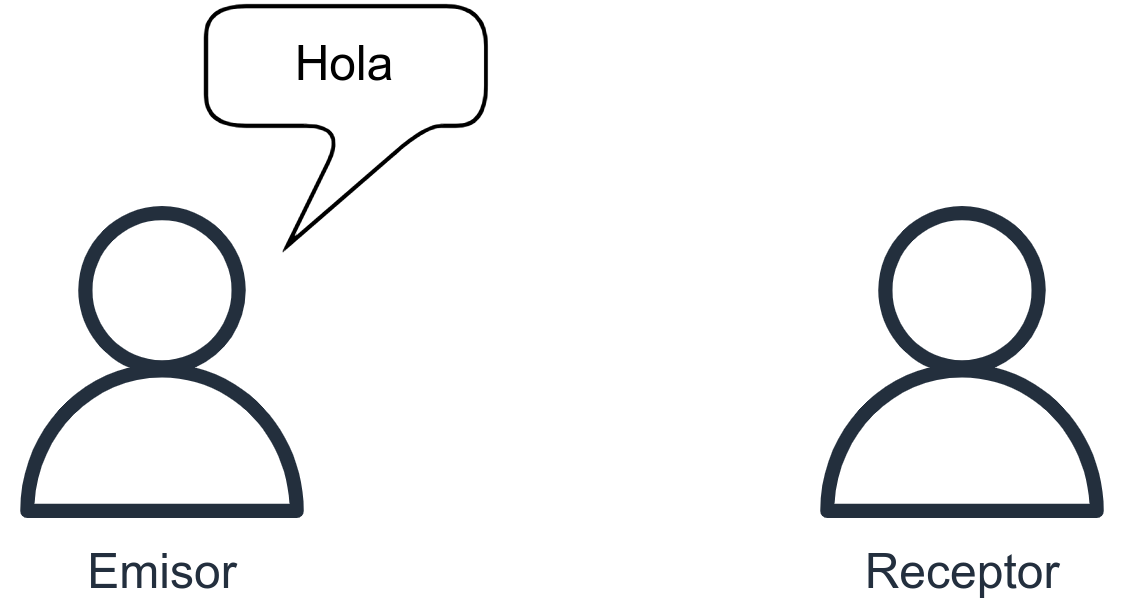
\includegraphics[width=\linewidth]{comunicacion-1.png}
    \vspace{-30pt}
\end{wrapfigure}
En este ejemplo vemos que hay dos personas, las cuales se han identificado cada una de ellas como “Emisor” y “Receptor”, y así de esta manera conocemos quién es el origen y quién el destino de la comunicación.

En este caso, el \textbf{mensaje} es “Hola”, haciendo uso del \textbf{código} conocido como “castellano”. La \textbf{señal} que se va a utilizar es la voz, ya que están hablando y el \textbf{canal} por el que se envía el mensaje es el aire.

Es un ejemplo sencillo que utilizamos cada día.

\subsubsection*{Ejemplo 2: Comunicación escrita por mensajería}

\begin{wrapfigure}{r}{0.25\linewidth}
    \centering
    \vspace{-35pt}
    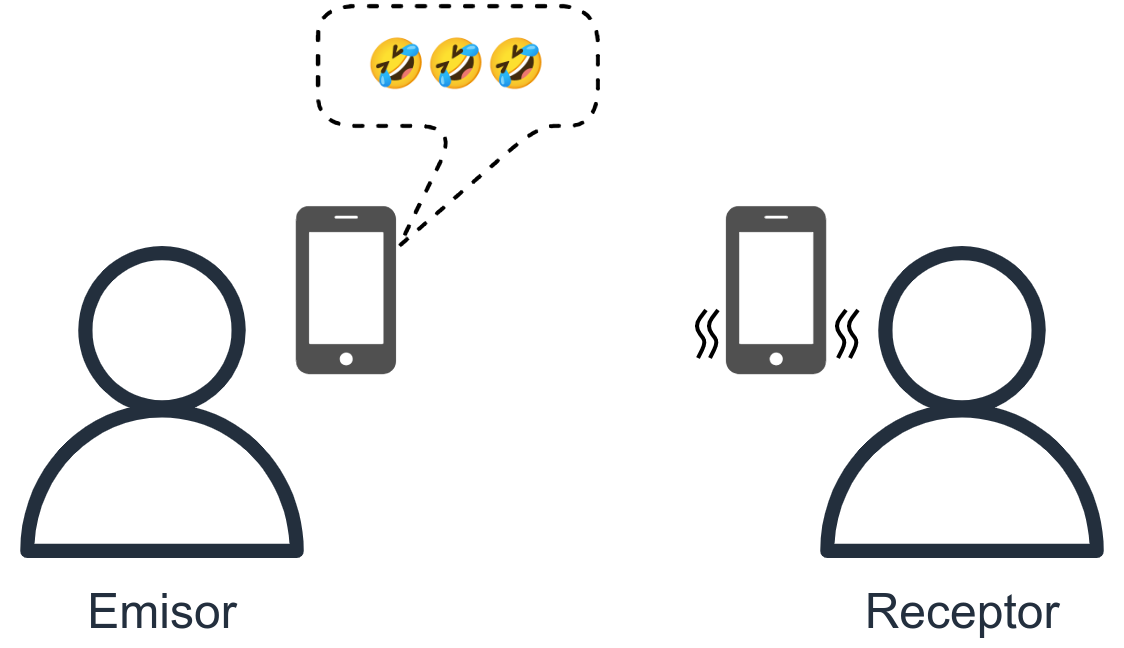
\includegraphics[width=\linewidth]{comunicacion-2.png}
    \vspace{-30pt}
\end{wrapfigure}
AL igual que en el ejemplo anterior, vemos que hay dos personas, las cuales se han identificado cada una de ellas como “Emisor” y “Receptor” pero que en este caso se van a comunicar haciendo uso de un teléfono móvil, tal como hacemos en nuestro día a día a través de una aplicación de mensajería o red social.

Teniendo en cuenta esto, en este ejemplo realmente existen dos sistemas de comunicación que están mezclados y uno está por encima del otro:

\begin{itemize}
    \item \textbf{Entre personas}: Similar al ejemplo anterior, el emisor y el receptor se están comunicando, con el mensaje compuesto por tres \href{https://es.wikipedia.org/wiki/Emoji}{emojis} que representan estar riendo. El \textbf{código} es el idioma que estén utilizando, el \textbf{canal} sería el programa utilizado y la \textbf{señal} podríamos decir que es el móvil.

    \item \textbf{Entre dispositivos}: En este caso, el emisor y receptor es el móvil de cada usuario. El mensaje es el mismo, pero convertido a un sistema digital (como el binario). El \textbf{canal} en este caso sería el aire y la \textbf{señal} es la utilizada por el móvil, por ejemplo 5G.
\end{itemize}

Tal como se puede ver en este caso, una comunicación puede depender a su vez de otro sistema de comunicación.


\section{Sistemas de numeración}
La información que queremos retransmitir debe estar representado de alguna manera, y tal como hemos visto previamente, \textbf{debe ser a través de un código que tanto emisor como receptor deben conocer}.

En sistemas orales, o escritos, lo habitual es hacer uso de un idioma concreto mediante un alfabeto conocido. En informática se hace uso de distintos sistemas de numeración para representar tanto números como el resto de información.

\subsection{Sistema decimal}
El ser humano, desde hace tiempo ha utilizado como sistema para contar el sistema decimal, que derivó del sistema indo-arábigo. Posiblemente se adoptó este sistema por contar con 10 dedos en las manos.

El sistema numérico decimal está basado en diez símbolos ordenados (0, 1, 2, 3, 4, 5, 6, 7, 8, 9), situados de manera ponderada (cada posición tiene un peso específico), que permiten representar las cantidades deseadas. Debido a que hacemos uso de diez símbolos se dice que utiliza la \textbf{base 10}.

\subsubsection*{Representación}
Cuando combinamos con otros sistemas de numeración, debemos indicar la base en la forma $ \mathbf{19_{(10}} $ , es decir, poniendo un pequeño “\textbf{(10}” a la derecha del número representado la base 10.

La representación de cualquier combinación del sistema decimal se puede representar en forma de potencia, donde la base es 10 (como ya hemos visto antes) y el exponente es la posición en la que se sitúa el símbolo.

Vamos a tomar como ejemplo el siguiente número: \textbf{146}. La representación en forma de potencias:

\begin{center}
    \vspace{-10pt}
    $ 146 =1\times10^2 + 4\times10^1 + 6\times10^0 $

    $ 146 = 1\times100 + 4\times10 + 6\times1 $

    $ 146 = 100+40+6 $
\end{center}

Como se puede comprobar, lo que hemos hecho ha sido coger cada símbolo representado y lo hemos multiplicado por la base (en este caso base 10) y a la base le hemos puesto el exponente de la posición en la que se encuentra. \textbf{El símbolo de más a la derecha tiene como exponente el cero}, y hacia la izquierda el exponente se incrementa en uno para cada posición.

\subsection{Sistema binario}

En informática el sistema binario es el más importante ya que es el sistema que internamente utilizan los circuitos digitales que configuran el hardware de las computadoras actuales. En este sistema sólo se hace uso de dos símbolos, el “0” y el “1”, y por tanto \textbf{su base es 2}. Los dos dígitos se denominan \textbf{bits} (contracción de \textbf{binary digit}).

\subsubsection*{Representación}

Para representar que estamos haciendo uso del sistema binario debemos indicar la base al lado del número, por ejemplo: $\mathbf{ 101001_{(2}} $. Como se puede ver es añadir “\textbf{(2}” en pequeño al final del último símbolo.


\subsection{Sistema hexadecimal}

En informática es muy habitual hacer uso del sistema hexadecimal a la hora de trabajar con \textbf{bytes} (que es una palabra de \textbf{8 bits}). Un símbolo hexadecimal se representa como 4 bits, por lo que necesitaríamos 2 símbolos hexadecimales para un byte.

También se usa durante la edición de código en formato de datos, o durante la programación en ensamblador.

Esta vez nos basamos en dieciséis símbolos ordenados, así que se dice que se hace uso de la \textbf{base 16}. Para la representación se hace uso de los símbolos digitales que conocemos (0, 1, 2, 3, 4, 5, 6, 7, 8, 9) y a continuación de las letras “A”, “B”, “C”, “D”, “E” y “F, de esta manera formamos los 16 símbolos que necesitamos.

\subsubsection*{Representación}
Al igual que con los sistemas anteriores, debemos añadir la base cuando estemos utilizando el sistema hexadecimal: $\mathbf{ F17A_{(16}} $ , $\mathbf{ FBE1D_{(16}} $ , $\mathbf{ 1FAB27_{(16}} $


\subsection{Sistema octal}
En ordenadores antiguos era habitual hacer uso del sistema octal. Hoy día se usa más como sistema intermedio entre binario y hexadecimal.

Esta vez nos basamos en ocho símbolos ordenados (0, 1, 2, 3, 4, 5, 6, 7), que, al combinarlos, permiten representar las cantidades deseadas. Debido a que hacemos uso de ocho símbolos se dice que utiliza la \textbf{base 8}.

\subsubsection*{Representación}
Para representar la base, debemos añadir “(8” a la derecha del número que hayamos indicado, como por ejemplo: $\mathbf{ 770_{(8} }$ , $\mathbf{ 175_{(8}} $


\subsection{Conversiones entre los distintos sistemas de numeración}

Hasta ahora no nos habíamos encontrado con distintos sistemas de numeración, pero ahora que conocemos cuatro de ellos, tenemos que saber que existe la posibilidad de realizar conversiones entre ellos.

Dependiendo del sistema de numeración de origen y cuál es el sistema de numeración al que queremos convertirlo, habrá que realizar una serie de pasos que pueden ser distintos.

Una vez entendidos los distintos sistemas de numeración nos tiene que quedar claro que aunque la representación de los símbolos sea la misma, el número o cantidad representada no es la misma. Por ejemplo:

\errorbox{
    \begin{center}
        $\mathbf{ 1010_{(10}  \neq  1010_{(2}  \neq  1010_{(16}  \neq 1010_{(8}} $
    \end{center}
}

A continuación se va a explicar cómo realizar conversiones entre los distintos sistemas de numeración que hemos visto, y a modo de resumen está la \hyperlink{tabla_conversiones_directas}{tabla de conversiones directa}.

\subsubsection{Conversión de decimal a...}
La manera más sencilla para realizar las distintas conversiones partiendo de un número decimal es hacer divisiones sucesivas usando la base a la que queremos realizar la conversión.

\subsubsection*{... binario}
Se trata de dividir sucesivamente el número decimal y los sucesivos cocientes entre dos (la base binaria).

Vamos a utilizar como ejemplo el número decimal $\mathbf{27_{(10}}$ :

\begin{center}
    \vspace{-20pt}
    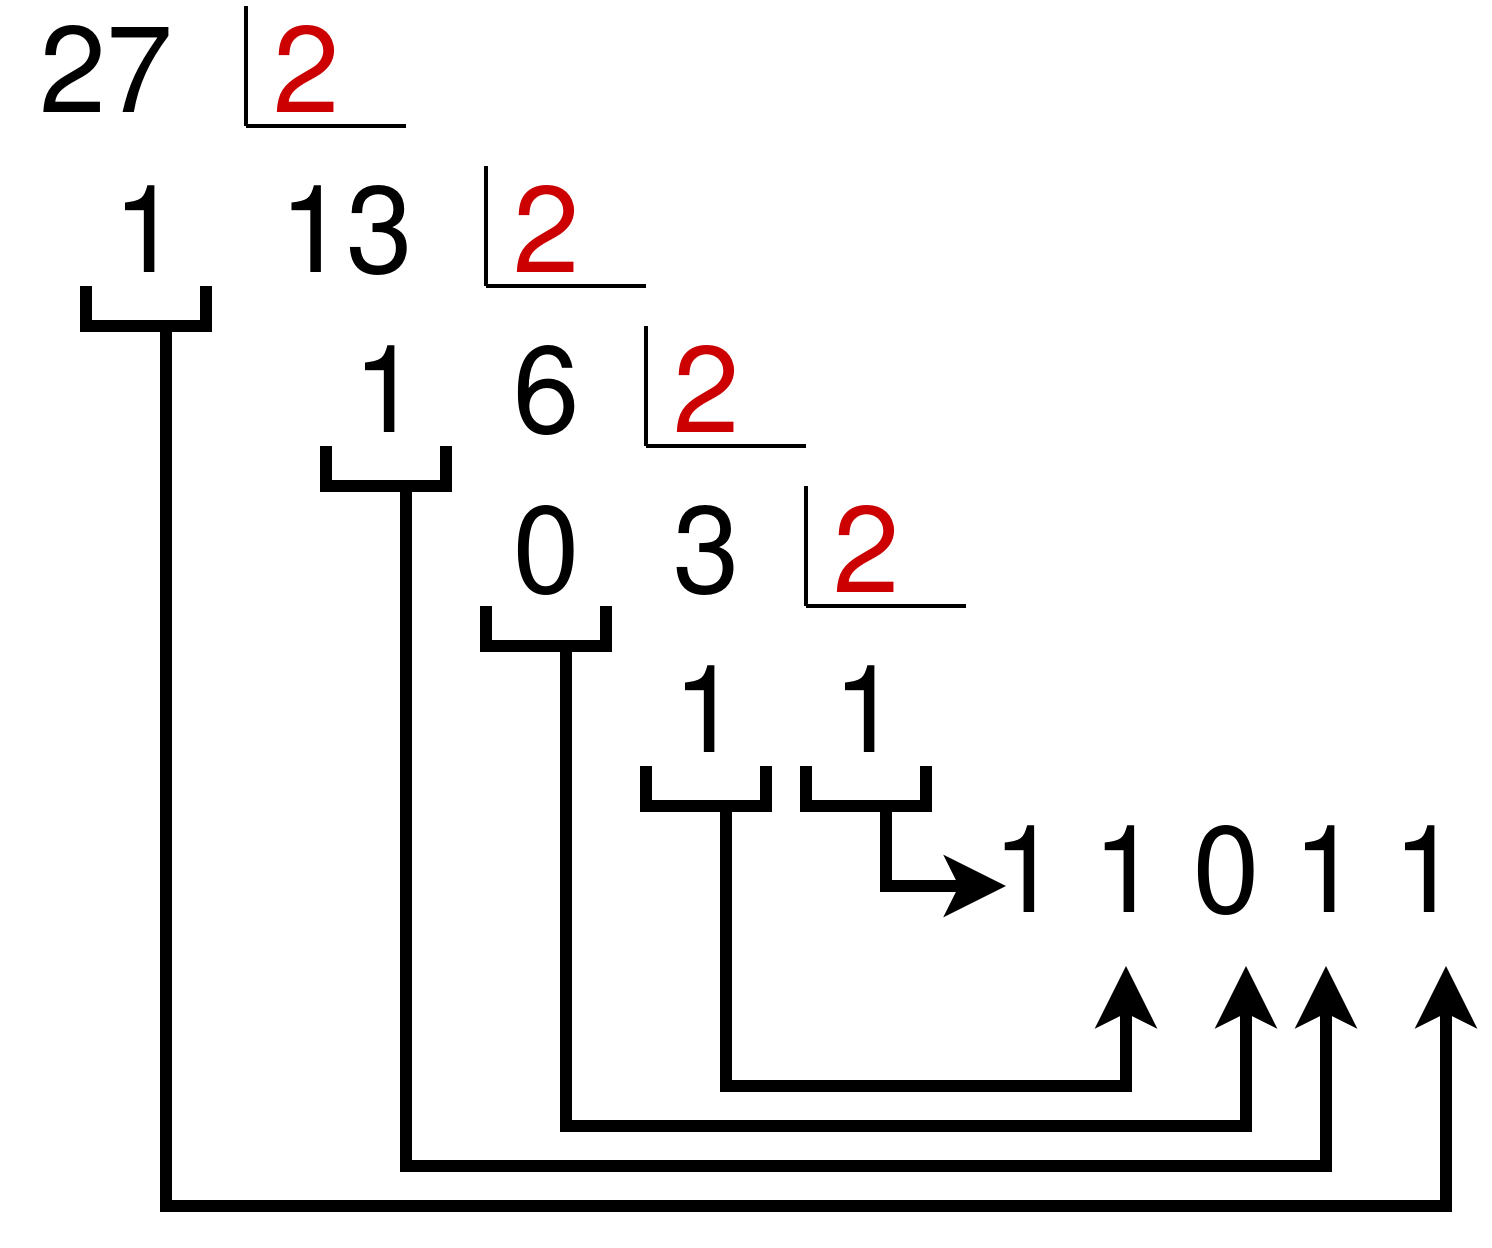
\includegraphics[width=0.29\linewidth]{decimal_binario.png}
    \vspace{-20pt}
\end{center}

De esta manera, podemos obtener la siguiente equivalencia: $\mathbf{27_{(10} = 11011_{(2}}$

\subsubsection*{... hexadecimal}
Se trata de dividir sucesivamente el número decimal y los sucesivos cocientes entre 16 (la base hexadecimal). Cuando el resultado sea entre 10 y 15, habrá que cambiarlo por la letra correspondiente.

\begin{center}
    \vspace{-10pt}
    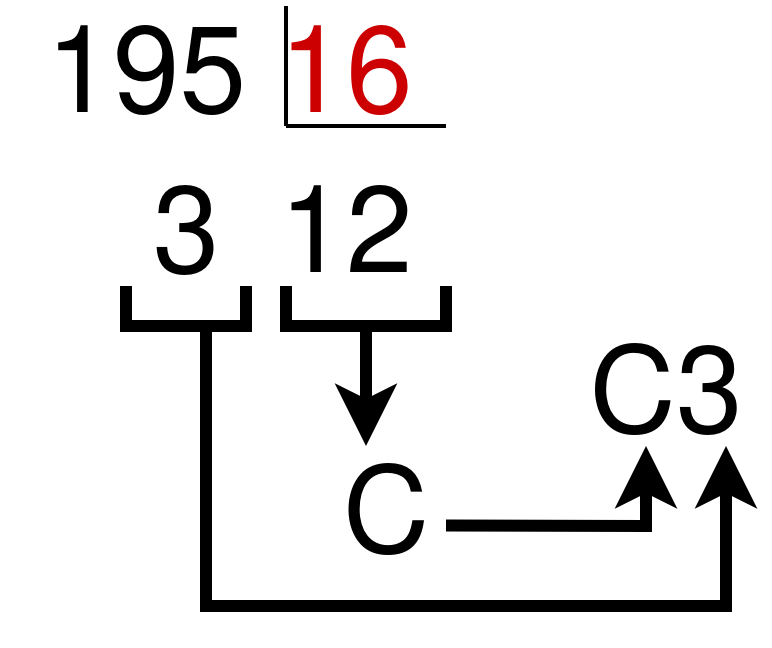
\includegraphics[width=0.2\linewidth]{decimal_hexadecimal.png}
    \vspace{-15pt}
\end{center}

De esta manera, podemos obtener la siguiente equivalencia: $\mathbf{195_{(10} = C3_{(16}}$

\subsubsection*{... octal}
Al igual que los anteriores, hacemos divisiones sucesivas:

\begin{center}
    \vspace{-10pt}
    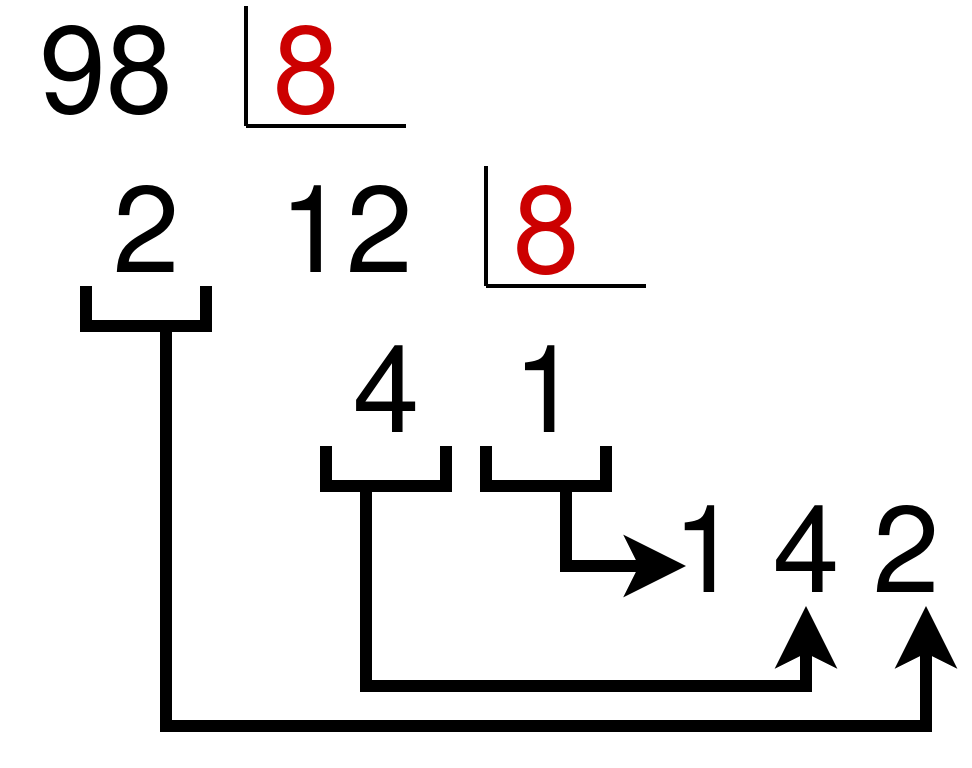
\includegraphics[width=0.25\linewidth]{decimal_octal.png}
    \vspace{-15pt}
\end{center}

De esta manera, podemos obtener la siguiente equivalencia: $\mathbf{98_{(10} = 142_{(8}}$


\subsubsection{Conversión de binario a...}

\subsubsection*{... decimal}
El sistema de numeración binario es un sistema posicional donde cada dígito binario (bit) tiene un valor basado en su posición relativa al \textbf{LSB} (\textit{Least Significant Bit} = bit menos significativo, que es el que está más a la derecha y que tiene el menor valor).

Cualquier número binario puede convertirse a su equivalente decimal, simplemente sumando en el número binario los valores de las diversas posiciones que contenga un 1. Para ilustrar lo anterior cojamos como ejemplo el número binario $\mathbf{11011_{(2}}$:

\begin{center}
    \vspace{-20pt}

    $ \mathbf{11011_{(2}} $

    $ \mathbf{1\times2^4 + 1\times2^3 + 0\times2^2 + 1\times2^1 + 1\times2^0} $

    $ \mathbf{16 + 8 + 0 + 2 + 1 = 27_{(10}} $
    \vspace{-15pt}
\end{center}

Nótese que el procedimiento consiste en determinar los valores (es decir, las potencias de 2) de cada posición de bit que contenga un 1 y luego sumarlos.

Nótese también que el \textbf{MSB} (\textit{Most Significant Bit} = bit más significativo, el que está más a la izquierda, el que tiene mayor valor) tiene un valor de $\mathbf{2^4}$ a pesar de que es el quinto bit. Esto se debe a que el \textbf{LSB} (\textit{Least Significant Bit}, el bit menos significativo, el que está a la derecha) es el primer bit y tiene un valor de $\mathbf{2^0}$.

\subsubsection*{... octal}
Para convertir un número binario a octal \textbf{se agrupan los dígitos de 3 en 3 desde el lado derecho hacia la izquierda}, sustituyendo cada trío de dígitos binarios por su equivalente en octal.

Si en el lado izquierdo quedase algún bit “suelto” (sin formar un grupo de 3), se pueden poner “0” a la izquierda.

Cogemos como ejemplo el número binario $\mathbf{1100101001001_{(2}}$ para pasarlo a octal, haremos:

\begin{center}
    \vspace{-15pt}
    $\mathbf{001\ \ 100\ \ 101\ \ 001\ \ 001_{(2} = 14511_{(10}}$
    \vspace{-15pt}
\end{center}

\subsubsection*{... hexadecimal}
Similar al caso anterior, pero en este caso \textbf{la agrupación que se realiza debe de ser de 4 en 4 bits}. Si usamos el mismo ejemplo anterior $\mathbf{1100101001001_{(2}}$ :

\begin{center}
    \vspace{-15pt}
    $\mathbf{0001\ \ 1001\ \ 0100\ \ 1001_{(2} = 1949_{(16}}$
    \vspace{-15pt}
\end{center}

\subsubsection{Conversión de hexadecimal a...}
\subsubsection*{... binario}
Para pasar de hexadecimal a binario convertiremos cada símbolo hexadecimal a 4 dígitos binarios.

\begin{center}
    \vspace{-15pt}
    $\mathbf{F17A_{(16} = 1111\ \ 0001\ \ 0111\ \ 1010_{(2}}$

    $\mathbf{1A4F_{(16} = 0001\ \ 1010\ \ 0100\ \ 111_{(2}}$
    \vspace{-15pt}
\end{center}


\subsubsection*{... decimal}
Al igual que hemos hecho con las conversiones previas a decimal, se podría realizar haciendo potencias de 16, pero se entiende que es más complicado de realizar.

Por lo tanto, \textbf{la manera más sencilla es pasar primero a binario} como acabamos de ver \textbf{y posteriormente convertir ese binario a decimal} como hemos visto previamente.

\subsubsection*{... octal}
Pasar primero a binario y después a octal.



\subsubsection{Conversión de octal a...}
\subsubsection*{... binario}
Cada dígito en octal se convierte en su representación en 3 bits:

\begin{center}
    \vspace{-15pt}
    $\mathbf{167_{(8} = 001\ \ 110\ \ 111_{(2}}$

    $\mathbf{253_{(8} = 010\ \ 101\ \ 011_{(2}}$
    \vspace{-15pt}
\end{center}
Los ceros de la izquierda se podrían quitar, ya que no alteran el valor.

\subsubsection*{... decimal}
Se puede realizar de dos maneras. La primera es hacer uso de potencias de 8 (similar al paso de pasar de binario a decimal, pero cambiando la base):

\begin{center}
    \vspace{-15pt}
    $\mathbf{157_{(8} = 1\times8^2 + 5\times8^1 + 7\times8^0 = }$

    $\mathbf{1\times64 + 5\times8 + 7\times1 = }$

    $\mathbf{64 + 40 + 7 = 111_{(10}}$

    Resultado: $\mathbf{157_{(8} = 111_{(10}}$
    \vspace{-15pt}
\end{center}

Con números grandes puede ser un poco complicado calcular las potencias de 8, por lo que \textbf{la alternativa es pasarlo primero a binario} como hemos visto, \textbf{y después pasarlo de binario a decimal}.

\subsubsection*{... hexadecimal}
La manera más sencilla es realizar la conversión primero a binario tal como hemos visto, y posteriormente pasar el número binario a hexadecimal como se ha visto previamente.


\chapter{Redes de comunicación}
En el ámbito informático una red de comunicaciones es representada como una red de ordenadores. Las redes de ordenadores son un conjunto de equipos hardware que están conectados entre sí (ya sea mediante cables o de manera inalámbrica) y que a través de un software especializado envían y reciben impulsos eléctricos (u ondas electromagnética) para el transporte de datos. De esta manera podrán compartir información, recursos u ofrecer servicios.

Al comienzo de las redes de ordenadores cada empresa creaba su propio sistema de comunicación creando su propio hardware y software, lo que hacía imposible la interconexión entre equipamiento de distintas empresas. Eso hoy en día no sucede ya que las redes están definidas en varios estándares, como veremos más adelante.

\section{Breve historia de las redes}
\begin{description}
    \item[\textasciitilde 1950]
    En la década de los 50 se desarrollan los circuitos integrados. Esto hará que en el futuro los ordenadores cada vez se vayan haciendo más pequeños.

    Las redes de ordenadores comienzan a aparecer en las bases militares americanas, en principio para sistemas de radares.

    \item[\char`\~ 1960]
    Se realiza una conexión entre dos mainframes en EEUU para el sistema de reservas aéreas comerciales.

    El \href{https://es.wikipedia.org/wiki/Instituto_de_Tecnolog%C3%ADa_de_Massachusetts}{MIT} utiliza un ordenador para enrutar y mantener conexiones telefónicas.

    En 1966, aparece un paper (artículo científico) describiendo las WAN.

    En 1969 ARPANET (red de ordenadores creadas por el Departamento de Defensa de Estados Unidos) cuenta con 4 nodos (a 50kbit/s de velocidad).

    \item[\char`\~ 1970]
    En 1972 se hace la primera demostración pública de ARPANET.

    A comienzos de la década (1973) se crea Ethernet en la compañía Xerox Parc.

    A finales de la década Xerox intenta hacer que Ethernet se convierta en un estándar de conexión para terminar con las competencias (token ring, …)
    Mapa de ARPANET en 1977 (Fuente: Wikipedia):

    \begin{center}
        \vspace{-10pt}
        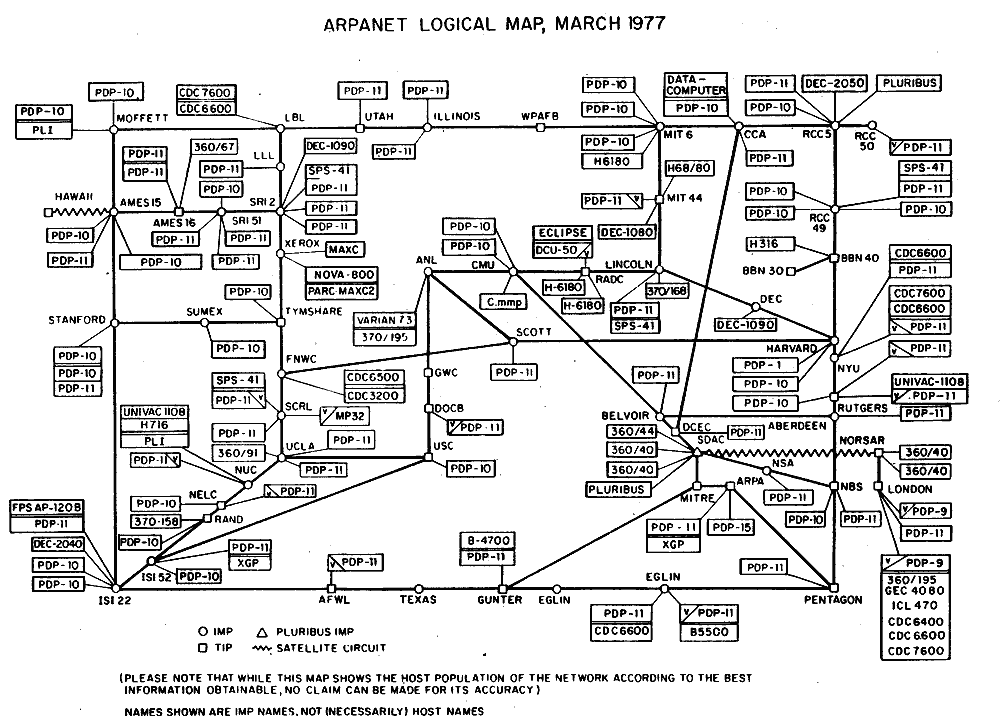
\includegraphics[frame,width=0.9\linewidth]{Arpanet_logical_map_march_1977.png}
        \vspace{-5pt}
        \captionof{figure}{Mapa lógico de ARPANET, marzo de 1977. Origen: \href{https://es.wikipedia.org/wiki/ARPANET\#/media/Archivo:Arpanet_logical_map,_march_1977.png}{ Wikipedia}}\vspace{-13pt}
    \end{center}

    \item[\char`\~ 1980]
    Los ordenadores personales empiezan a generalizarse.

    Aparece el protocolo para enviar y recibir e-mails (SMTP).

    El protocolo TCP/IP se convierte en el utilizado por ARPANET (1983) y es declarado como su estándar para las comunicaciones.

    Aparece el servicio DNS.

    Se crea el modelo de referencia OSI.

    Aparece el primer gusano por la red (Morris worm, 1988). Se estima que infectó al 10\% de los ordenadores conectados a la red.

    Se crea el protocolo BGP.

    El protocolo Ethernet evoluciona y permite conexiones a 10Mbit/s.


    \item[\char`\~ 1990]
    Tim Berners-Lee desarrolla el código para WWW y crea el primer servidor web (1991).

    Se puede decir que aquí es cuando nace la Internet que conocemos actualmente.

    En 1995 Ethernet permite conexiones a 100Mbit/s

    Se establece un control para los nombres de dominio (posteriormente lo asumirá ICANN).

    Aparece Amazon, ebay, Craiglist, IMDB, hotmail, google, yahoo, ...

    Aparece el protocolo IPv6 (1998).

    Aparece el protocolo wifi 802.11b.

    \item[\char`\~ 2000]
    Crisis de las “.com”.

    Internet se generaliza.

    Empiezan a permitirse más TLDs, que no corresponden sólo a países.

    Ethernet permite conexiones a 1Gbit/s

    \item[\char`\~ 2010]
    Ethernet permite conexiones a 400Gbit/s (2018).

    Starlink comienza a desplegar su constelación de satélites para dar cobertura en todo el planeta.


\end{description}






\section{Sistemas de transmisión}



\section{Arquitectura en capas}



\section{Modelo de referencia OSI}


\section{Arquitectura TCP/IP}





\chapter{Conexión de redes a nivel físico}






\chapter{Conexión de redes a nivel de enlace de datos}


\section{Administración de switches}



\chapter{Interconexión de redes}

\section{Encaminamiento de tráfico}

\subsection{Puerta de enlace (gateway)}

\subsection{NAT}


\subsection{Rutas estáticas}


\subsection{Enrutamiento dinámico}

\subsubsection{BGP (Border Gateway Protocol)}



\section{Administración de routers}









\chapter{Redes virtuales}

\section{VLANs}

\section{Protocolo VTP}



\chapter{Alta Disponibilidad en sistemas de red}

\section{Stack de switches}

\section{Agregación de enlaces: Etherchannel / LACP}